% 18 variables in here:
% h_1 = 10.0, h_2 = 10.0, h_3 = 10.0, h_4 = 10.0, h_5 = 10.0, h_6 = 10.0, ux_1 = 0.0, ux_2 = 1.0, ux_3 = 1.0, ux_4 = 1.0, ux_5 = 1.0, ux_6 = 1.0, uy_1 = 0.0, uy_2 = 0.0, uy_3 = 0.0, uy_4 = 0.0, uy_5 = 0.0, uy_6 = 0.0
\begin{figure}[ht!]
\centering
  \subfloat[$SE_x^1$] {
    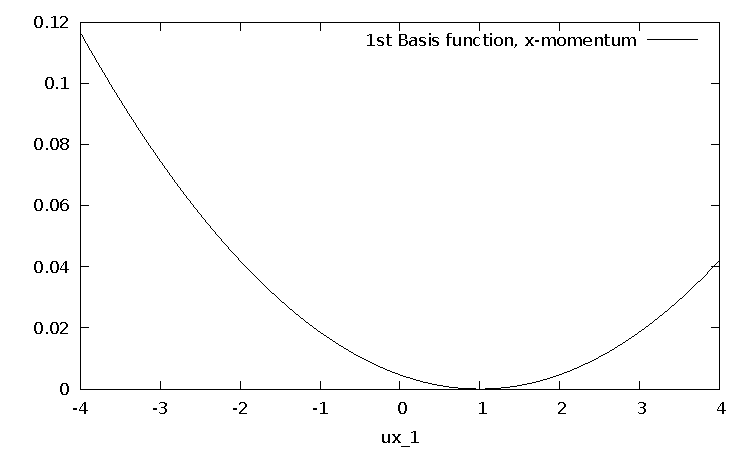
\includegraphics[scale=\zoomfactor]{{{ord2_varying_ux1_ux2-ux6_1/10.0_10.0_10.0_10.0_10.0_10.0_y_1.0_1.0_1.0_1.0_1.0_0.0_0.0_0.0_0.0_0.0_0.0f00}}}
  }
  % \subfloat[] {
  %   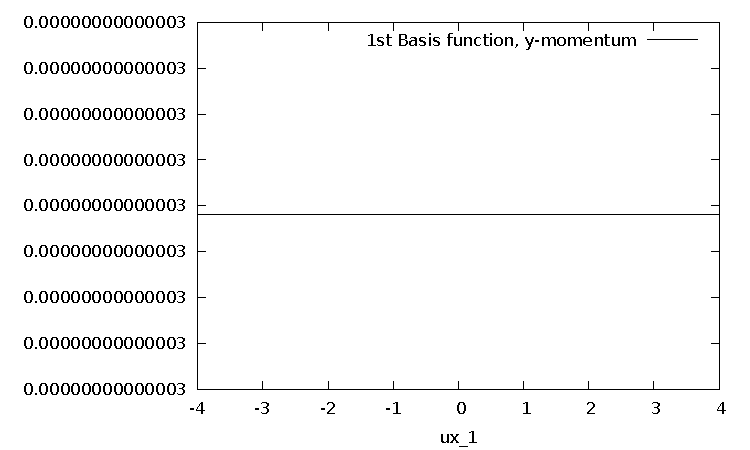
\includegraphics[scale=\zoomfactor]{{{ord2_varying_ux1_ux2-ux6_1/10.0_10.0_10.0_10.0_10.0_10.0_y_1.0_1.0_1.0_1.0_1.0_0.0_0.0_0.0_0.0_0.0_0.0f01}}}
  % }
  \subfloat[$SE_x^2$] {
    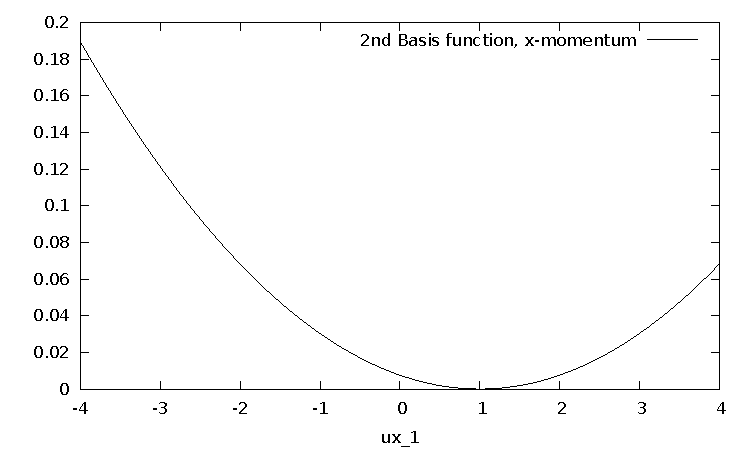
\includegraphics[scale=\zoomfactor]{{{ord2_varying_ux1_ux2-ux6_1/10.0_10.0_10.0_10.0_10.0_10.0_y_1.0_1.0_1.0_1.0_1.0_0.0_0.0_0.0_0.0_0.0_0.0f02}}}
  }
  % \subfloat[] {
  %   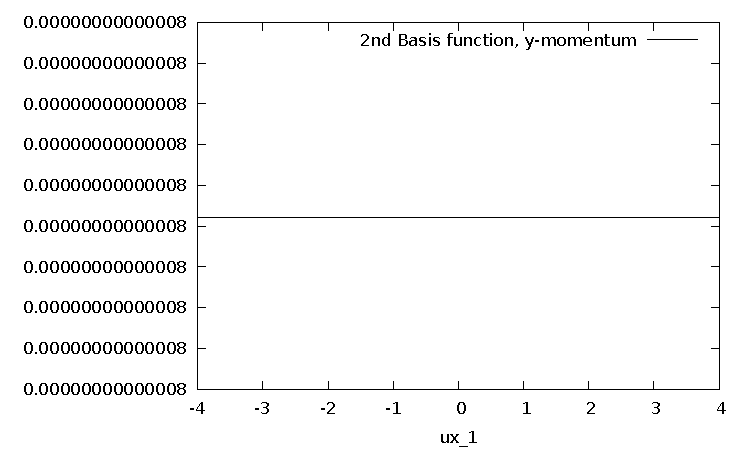
\includegraphics[scale=\zoomfactor]{{{ord2_varying_ux1_ux2-ux6_1/10.0_10.0_10.0_10.0_10.0_10.0_y_1.0_1.0_1.0_1.0_1.0_0.0_0.0_0.0_0.0_0.0_0.0f03}}}
  % }
  \subfloat[$SE_x^3$] {
    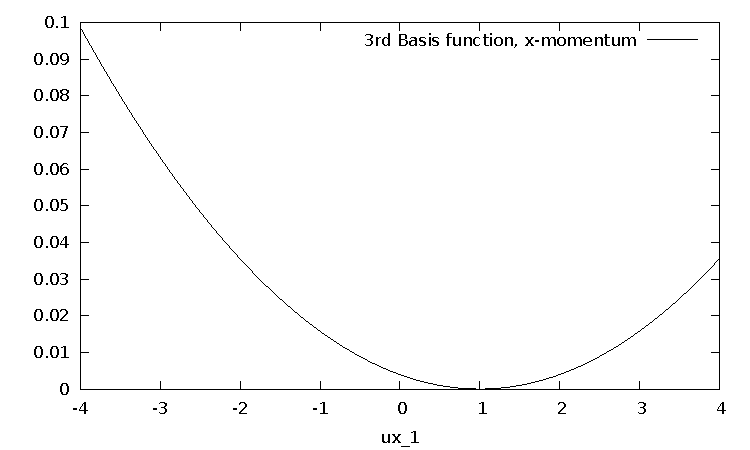
\includegraphics[scale=\zoomfactor]{{{ord2_varying_ux1_ux2-ux6_1/10.0_10.0_10.0_10.0_10.0_10.0_y_1.0_1.0_1.0_1.0_1.0_0.0_0.0_0.0_0.0_0.0_0.0f04}}}
  }
  % \subfloat[] {
  %   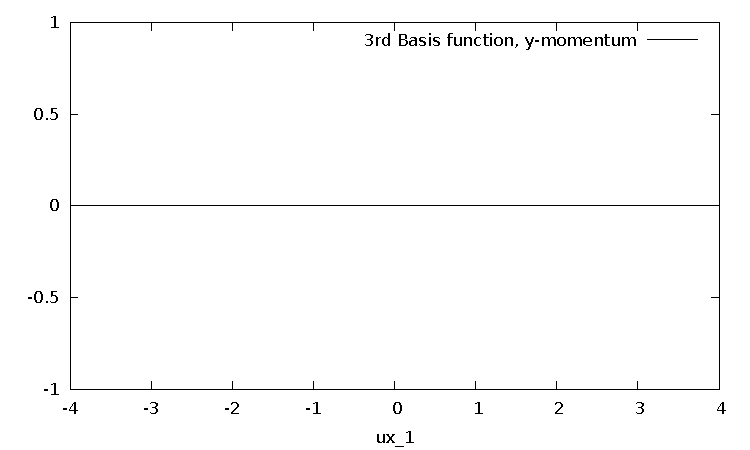
\includegraphics[scale=\zoomfactor]{{{ord2_varying_ux1_ux2-ux6_1/10.0_10.0_10.0_10.0_10.0_10.0_y_1.0_1.0_1.0_1.0_1.0_0.0_0.0_0.0_0.0_0.0_0.0f05}}}
  % }
  \subfloat[$SE_x^4$, $SE_x^6$] {
    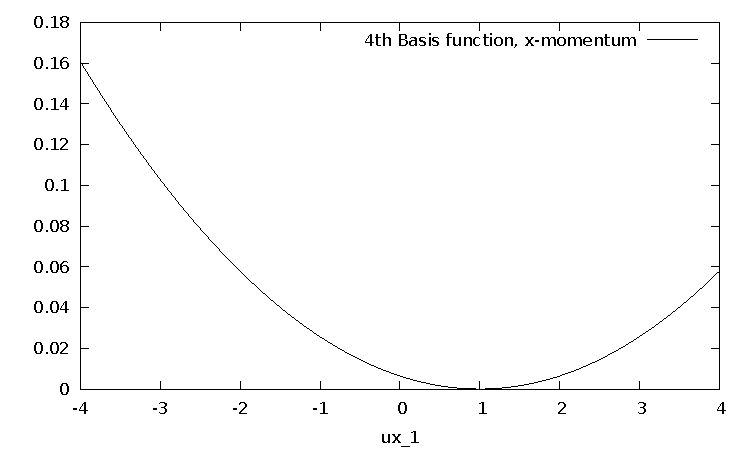
\includegraphics[scale=\zoomfactor]{{{ord2_varying_ux1_ux2-ux6_1/10.0_10.0_10.0_10.0_10.0_10.0_y_1.0_1.0_1.0_1.0_1.0_0.0_0.0_0.0_0.0_0.0_0.0f06}}}
  }
  % \subfloat[] {
  %   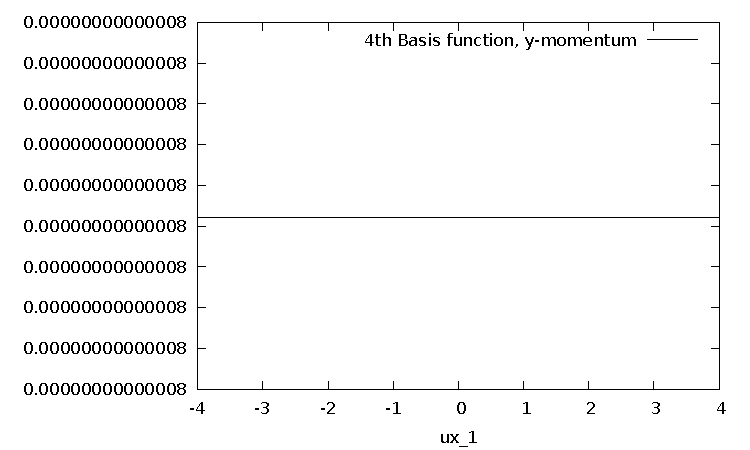
\includegraphics[scale=\zoomfactor]{{{ord2_varying_ux1_ux2-ux6_1/10.0_10.0_10.0_10.0_10.0_10.0_y_1.0_1.0_1.0_1.0_1.0_0.0_0.0_0.0_0.0_0.0_0.0f07}}}
  % }
  % \subfloat[$SE_x^5$, $SE_y^i$ for all basis functions] {
  %   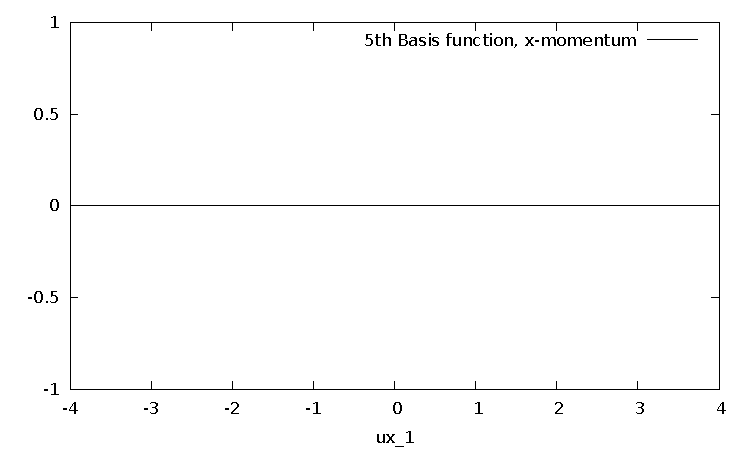
\includegraphics[scale=\zoomfactor]{{{ord2_varying_ux1_ux2-ux6_1/10.0_10.0_10.0_10.0_10.0_10.0_y_1.0_1.0_1.0_1.0_1.0_0.0_0.0_0.0_0.0_0.0_0.0f08}}}
  % }
  % \subfloat[] {
  %   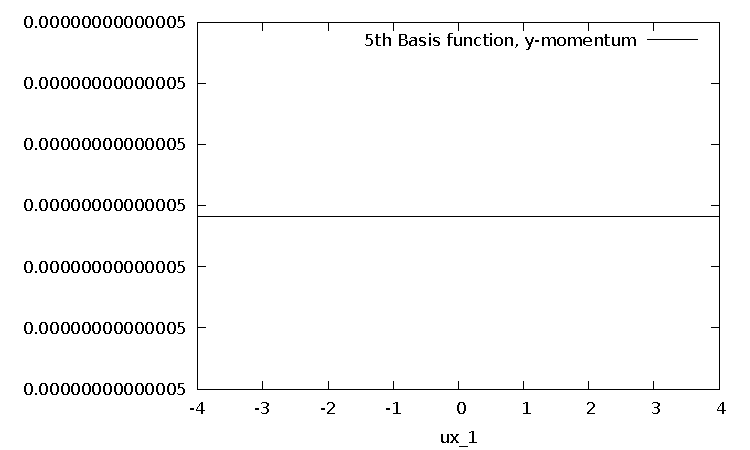
\includegraphics[scale=\zoomfactor]{{{ord2_varying_ux1_ux2-ux6_1/10.0_10.0_10.0_10.0_10.0_10.0_y_1.0_1.0_1.0_1.0_1.0_0.0_0.0_0.0_0.0_0.0_0.0f09}}}
  % }
  % \subfloat[$SE_x^6$] {
  %   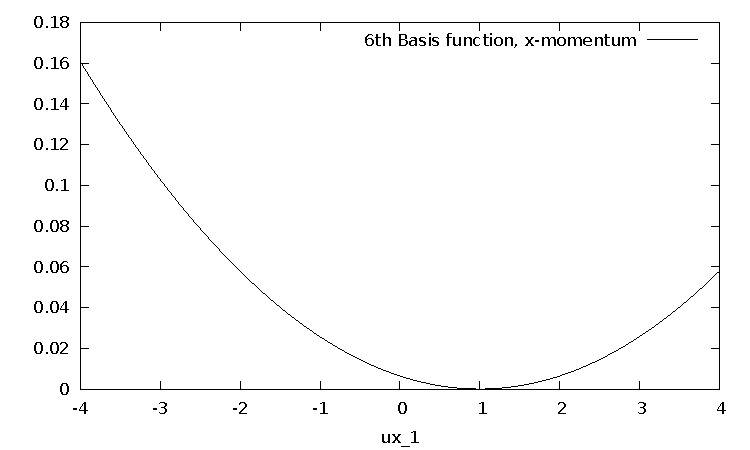
\includegraphics[scale=\zoomfactor]{{{ord2_varying_ux1_ux2-ux6_1/10.0_10.0_10.0_10.0_10.0_10.0_y_1.0_1.0_1.0_1.0_1.0_0.0_0.0_0.0_0.0_0.0_0.0f10}}}
  % }
  % \subfloat[] {
  %   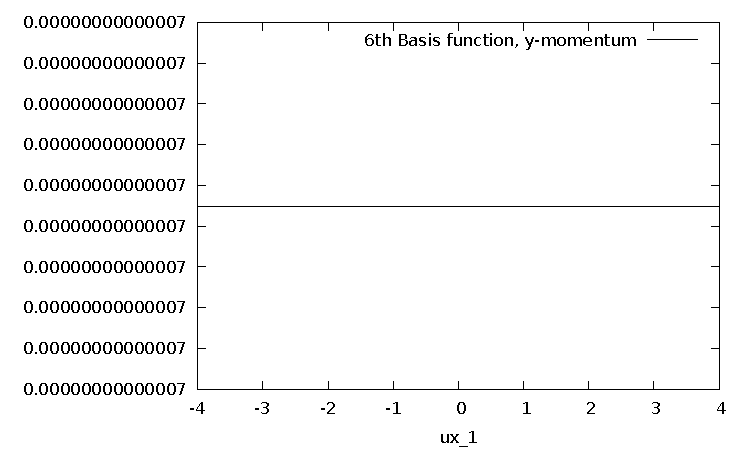
\includegraphics[scale=\zoomfactor]{{{ord2_varying_ux1_ux2-ux6_1/10.0_10.0_10.0_10.0_10.0_10.0_y_1.0_1.0_1.0_1.0_1.0_0.0_0.0_0.0_0.0_0.0_0.0f11}}}
  % }
\caption{Errors for second order. All $x$-momentums are set to 1, and all $y$-momentums to 0. All heights are 10. We see -- as expected -- perfect-looking parabolae that reach a minimum error of 0 at $u_{x,1}=1$. $SE_x^5$ and all $SE_y^i$ have been omitted since they are zero.}
\label{fig:ord2_varying_ux1_ux2-ux6_1}
\end{figure}

%%% Local Variables:
%%% TeX-master: "../results.tex"
%%% End:
